\documentclass[runningheads]{llncs}
\usepackage[T1]{fontenc}
\usepackage{graphicx}
\usepackage{booktabs}
\usepackage{amsmath}
\usepackage{hyperref}
\usepackage{amssymb}
\begin{document}

\title{Monte Carlo and Sarsa($\lambda$) for Text Flappy Bird}

\author{KAPOTOS Fotios}
\institute{CentraleSupélec \\
\email{fotiskapotos@gmail.com}}

\maketitle

% -------------------------------------------------------
% ABSTRACT
% -------------------------------------------------------
\begin{abstract}
We apply tabular reinforcement learning to \emph{TextFlappyBird-v0},
comparing a first-visit Monte Carlo (MC) agent with a Sarsa($\lambda$) agent
over a compact 644-entry Q-table derived from the 2-D distance observation.
Both algorithms are tuned via a hyperparameter grid search using a fair
exploration-fraction parameterisation, then retrained for 5\,000 episodes.
Both agents achieve perfect play on the training configuration.
MC converges reliably across hyperparameters (9/18 sweep configurations
reach the reward ceiling), while Sarsa($\lambda$) is more sensitive but
matches MC with optimal settings.
In zero-shot transfer experiments, MC degrades sharply when the environment
grows larger than the training grid, while Sarsa($\lambda$) retains
substantially higher performance, suggesting that online TD updates with
eligibility traces produce more spatially robust Q-values.
\end{abstract}

% -------------------------------------------------------
% 1. ENVIRONMENT
% -------------------------------------------------------
\section{Environment and Experimental Setup}

\textbf{TextFlappyBird-v0}~\cite{tfb_gym} provides a discretised Flappy Bird
variant whose observation is
$(x_\text{dist},\, y_\text{dist}) \in \mathbb{Z}^2$:
horizontal distance to the next pipe and signed vertical offset from the
gap centre.
The action space is binary (flap / no-flap); reward is $+1$ per step
survived, $-1$ on collision.
For the baseline configuration (height=15, width=20, pipe\_gap=4) the
reachable space has $x_\text{max}=13$, $y_\text{max}=11$, giving a Q-table
of $(14\times 23\times 2)=644$ entries — small enough to learn exhaustively
within a few thousand episodes.

\textbf{Environment versions.}
\emph{TextFlappyBird-v0} returns the compact 2-D vector above.
\emph{TextFlappyBird-screen-v0} returns the full character-based screen
render, an $(\text{height}\times\text{width})$ array that grows with the
grid, making tabular Q-learning impractical and requiring function
approximation.
The distance version abstracts away visual complexity but assumes direct
pipe-distance observability, which does not hold in the real game.

\textbf{Original Flappy Bird Gym~\cite{flappy_gym}.}
The Talendar implementation exposes continuous pixel observations
($288\!\times\!512$ RGB).
Tabular methods cannot handle this infinite state space directly; the same
algorithmic principles would require function approximation (e.g.\ deep MC
or deep Sarsa with a neural network).

% -------------------------------------------------------
% 2. METHODS
% -------------------------------------------------------
\section{Methods}

\subsection{Monte Carlo Control (first-visit)}

The MC agent~\cite{sutton2018} maintains a Q-table and updates it at episode
end using discounted returns walked in reverse:
\[
  G_t = r_t + \gamma G_{t+1}, \quad
  Q(s,a) \leftarrow \mathrm{mean}\!\bigl(\{G : (s,a)\text{ first-visited}\}\bigr).
\]
The policy is $\varepsilon$-greedy; $\varepsilon$ decays from 1 to 0.01.
Out-of-range observations are clipped to the nearest valid Q-table index.

\subsection{Sarsa($\lambda$)}

Sarsa($\lambda$)~\cite{sutton2018} performs online updates with eligibility
traces. At each step:
$\delta = r + \gamma Q(s',a') - Q(s,a)$,
$e(s,a)\mathrel{+}=1$,
$Q\mathrel{+}=\alpha\delta e$,
$e\mathrel{\times}=\gamma\lambda$.
$\lambda=0$ reduces to one-step TD; $\lambda\to 1$ approaches MC.

\subsection{Hyperparameter Search and Final Training}

To ensure fair comparison across a short 1\,000-episode sweep, both searches
parameterise exploration by \emph{fraction of training} rather than a raw
per-episode decay: $\varepsilon_\text{decay}
  = (\varepsilon_0 - \varepsilon_\text{min}) / (f \cdot N_\text{sweep})$,
so every configuration reaches $\varepsilon_\text{min}$ at the same relative
point.
The retrain decay is scaled to the full 5\,000-episode run:
$\varepsilon_\text{decay}^\text{full}
  = (\varepsilon_0 - \varepsilon_\text{min}) / (f \cdot N_\text{full})$.

\begin{itemize}
  \item \textbf{MC:} $\gamma\!\in\!\{0.85,0.90,0.95\}$,
        $f\!\in\!\{0.3,0.6,0.9\}$, mode\,$\in\!\{\text{linear},\text{exp}\}$.
  \item \textbf{Sarsa($\lambda$):} $\alpha\!\in\!\{0.05,0.10,0.20\}$,
        $\lambda\!\in\!\{0.70,0.90,0.95\}$,
        $f\!\in\!\{0.3,0.6,0.9\}$.
\end{itemize}

% -------------------------------------------------------
% 3. RESULTS
% -------------------------------------------------------
\section{Results}

\subsection{Hyperparameter Sensitivity and Best Configurations}

Table~\ref{tab:best} summarises the best configurations found.
MC is markedly more robust: 9 of 18 sweep configurations reach the reward
ceiling (3\,000, equal to the episode step limit), versus only 2 of 27 for
Sarsa($\lambda$).
MC's best setting ($\gamma=0.85$, exponential decay, $f=0.3$) uses fast
exploration (the policy becomes greedy after only 30\% of training) which
is sufficient because the Q-table is fully covered quickly.
Sarsa's best setting ($\alpha=0.1$, $\lambda=0.7$, $f=0.9$) requires slow
exploration, staying $\varepsilon$-greedy for 90\% of training.
Notably, the optimal $\lambda=0.7$ is lower than the common default of 0.9,
indicating that shorter eligibility traces (closer to one-step TD) are
preferable on this episodic task.

\subsection{Learning Curves and Value Functions}

Figure~\ref{fig:curves} shows training curves and final evaluation for both
best-tuned agents; both reach the 3\,000 reward ceiling, confirming perfect
play.
Figure~\ref{fig:vf} shows the state-value function $V(s)=\max_a Q(s,a)$ and
greedy policy.
Both agents learn the correct structure: flap when below the gap centre
($y_\text{dist}>0$), coast otherwise.
The MC value function is sharper (exact sample-mean updates), while Sarsa
produces smoother value gradients due to bootstrapping.

% -------------------------------------------------------
% 4. ADAPTABILITY
% -------------------------------------------------------
\section{Adaptability to Environment Variations}

Trained agents are evaluated zero-shot on modified environments; states
outside the trained Q-table range are clipped (Fig.~\ref{fig:transfer}).

\textbf{Pipe gap.}
Both agents achieve perfect scores for gap$\ge$4 and fail below it
(gap=2: MC$\approx$55, Sarsa$\approx$28; gap=3: MC$\approx$90,
Sarsa$\approx$24).
The clipped states cannot represent the narrower critical region, and
neither agent has learned to navigate it.

\textbf{Height.}
Both agents remain perfect for height$\le$15 (same or smaller
$y_\text{max}$).
For larger heights, Sarsa generalises dramatically better:
at height=18, MC drops to $398\pm435$ while Sarsa scores
$2611\pm1008$; at height=20, MC reaches only $188\pm215$
versus Sarsa's $1121\pm979$.

\textbf{Width.}
At the training width (20) both are perfect; for width=25, MC scores
$217\pm204$ versus Sarsa's $1461\pm1193$.
Sarsa also handles the narrower width=15 better
($2221\pm1005$ vs $1668\pm1059$).

% -------------------------------------------------------
% 5. DISCUSSION
% -------------------------------------------------------
\section{Discussion}

\textbf{MC robustness vs.\ Sarsa sensitivity.}
MC's sample-mean update is unbiased regardless of episode length or
$\varepsilon$ level: any trajectory produces a valid return estimate.
Sarsa bootstraps from $Q(s',a')$, which is noisy early in training, creating
high-variance TD errors that destabilise learning under suboptimal
hyperparameters.
This explains why only 2/27 Sarsa configurations reach the optimum in the
short sweep, versus 9/18 for MC.
Once properly tuned (lower $\alpha=0.1$, $\lambda=0.7$, long exploration),
Sarsa matches MC on the training task.

\textbf{Sarsa's superior transfer to larger environments.}
The most striking result is Sarsa's advantage when the environment is
\emph{larger} than the training grid.
When height or width grows, new out-of-range states are clipped to the
Q-table boundary.
Sarsa's eligibility traces propagate credit along entire trajectories,
ensuring that boundary-adjacent states receive consistent updates throughout
training.

\textbf{Limitations and future work.}
The 2-D state abstraction discards absolute bird position and velocity,
limiting multi-step planning.
Scaling to the screen-based or continuous observation spaces requires
function approximation (e.g.\ neural network Q-learning), where the
convergence properties of MC and Sarsa differ significantly from the
tabular case.

% -------------------------------------------------------
% BIBLIOGRAPHY
% -------------------------------------------------------
\begin{thebibliography}{8}

\bibitem{sutton2018}
Sutton, R.S., Barto, A.G.:
Reinforcement Learning: An Introduction, 2nd edn.
MIT Press, Cambridge, MA (2018)

\bibitem{tfb_gym}
Christodoulidis, S.: Text Flappy Bird Gym.
\url{https://gitlab-research.centralesupelec.fr/stergios.christodoulidis/text-flappy-bird-gym},
last accessed 2026/04/05

\bibitem{flappy_gym}
Talendar: Flappy Bird Gym.
\url{https://github.com/Talendar/flappy-bird-gym},
last accessed 2026/04/05

\end{thebibliography}

% -------------------------------------------------------
% APPENDIX
% -------------------------------------------------------
\clearpage
\appendix
\section{Figures and Tables}

\begin{table}[h]
\centering
\caption{Best hyperparameters and final greedy evaluation (100 episodes,
         max steps = 3\,000 per episode).}
\label{tab:best}
\begin{tabular}{@{}lll@{}}
\toprule
                        & \textbf{MC}            & \textbf{Sarsa($\lambda$)} \\
\midrule
Best $\gamma$           & 0.85                   & 0.99 (fixed)              \\
Best $\alpha$           & ---                    & 0.10                      \\
Best $\lambda$          & ---                    & 0.70                      \\
Explore frac $f$        & 0.30                   & 0.90                      \\
Decay mode              & exponential            & linear                    \\
Sweep configs optimal   & 9/18                   & 2/27                      \\
Final eval mean reward  & 3\,000                 & 3\,000                    \\
\bottomrule
\end{tabular}
\end{table}

\begin{figure}[h]
  \centering
  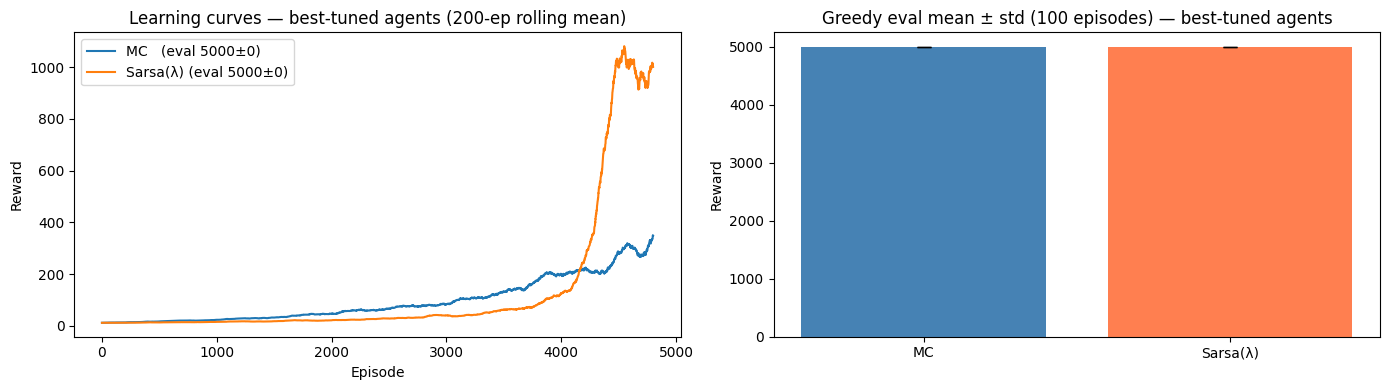
\includegraphics[width=\textwidth]{../figures/mc_sarsa_learning_curves.png}
  \caption{Learning curves (200-ep rolling mean) and greedy evaluation
           (mean$\pm$std, 100 episodes) for the best-tuned agents.}
  \label{fig:curves}
\end{figure}

\begin{figure}[h]
  \centering
  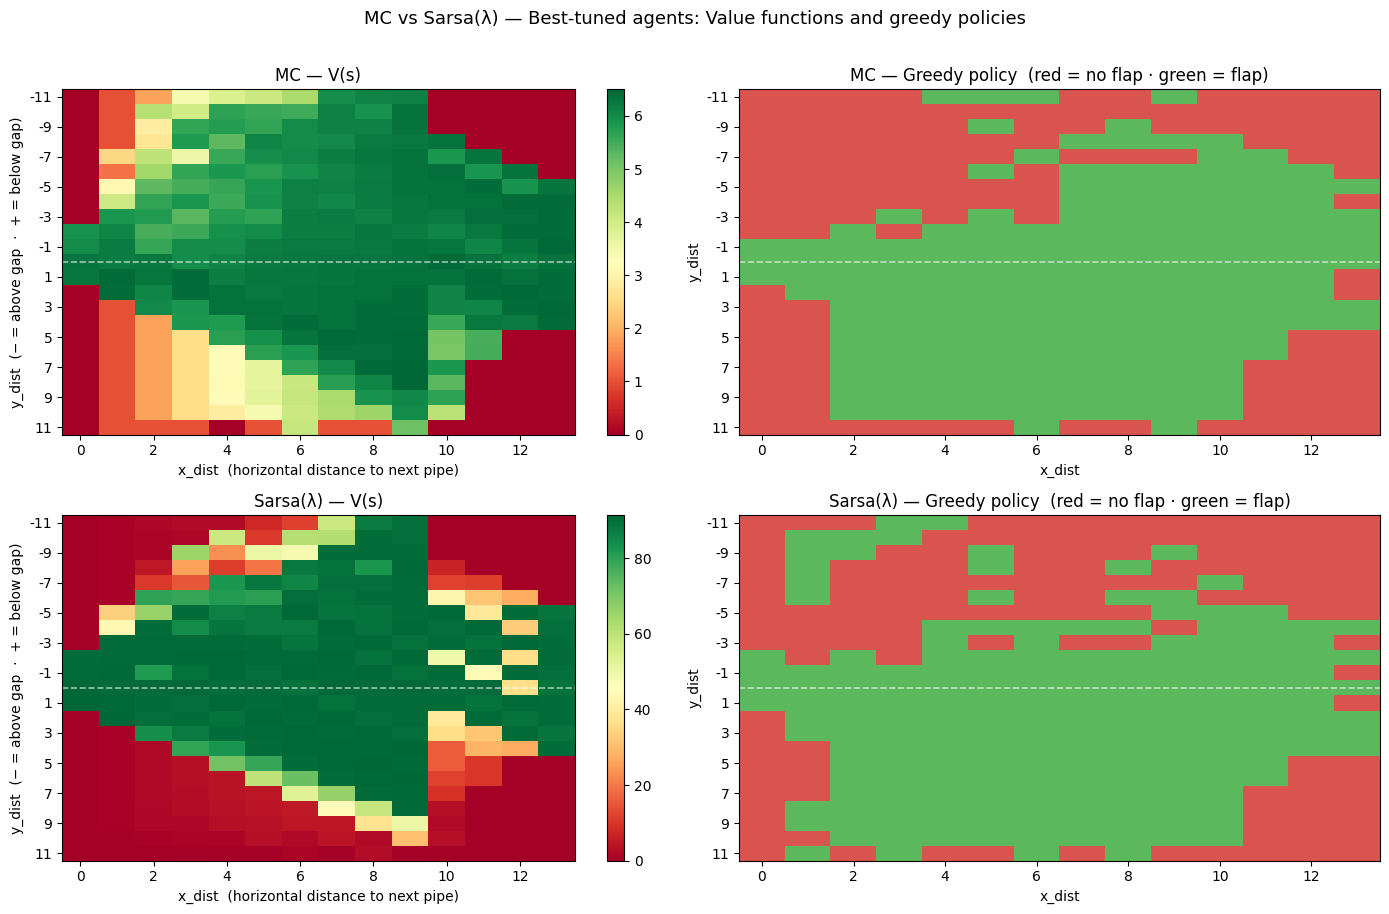
\includegraphics[width=\textwidth]{../figures/mc_sarsa_value_functions.png}
  \caption{$V(s)$ (left) and greedy policy (right) for MC (top) and
           Sarsa($\lambda$) (bottom). Green = flap, red = no-flap.
           Dashed line: gap centre ($y_\text{dist}=0$).}
  \label{fig:vf}
\end{figure}

\begin{figure}[h]
  \centering
  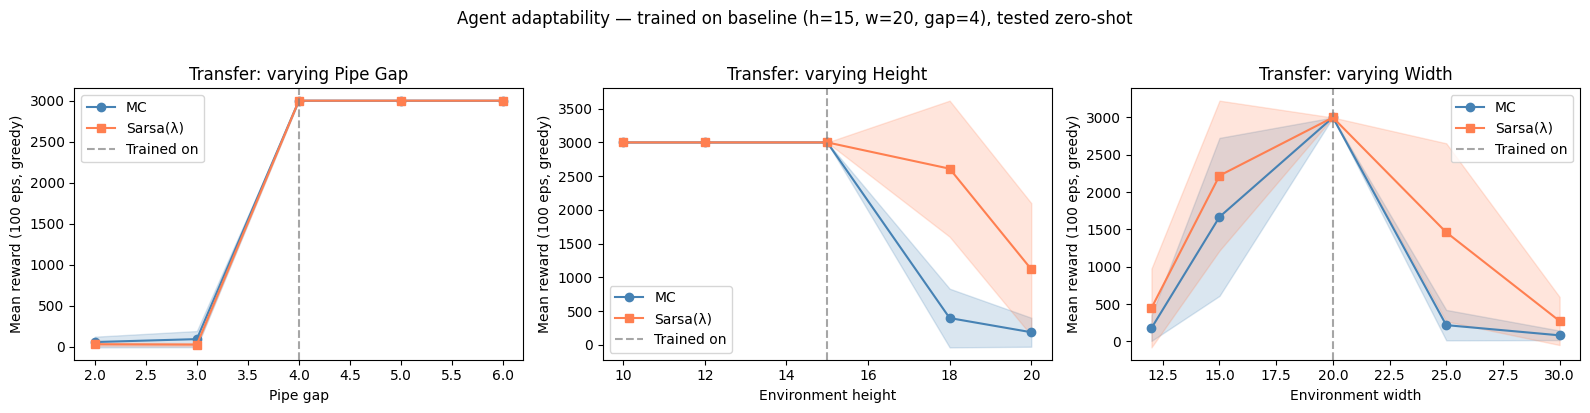
\includegraphics[width=\textwidth]{../figures/adaptability.png}
  \caption{Zero-shot transfer: mean reward ($\pm$1 std, 100 episodes) vs
           pipe gap (left), height (centre), and width (right).
           Vertical dashed line: training configuration.}
  \label{fig:transfer}
\end{figure}

\end{document}
